\preClass{Coordinate Systems}



\noindent Watch the Pre-Class videos for Section 3.1 and answer the following questions. Remember that in your written work you are graded on the correctness of your supporting work and not just your final answer. Always give an exact answer unless you are explicitly told to round; calculator approximations will not receive full credit.


\begin{enumerate}

\item  Determine if $f(x)=-4x+1$ is one-to-one both algebraically and graphically.
\begin{enumerate}

\item  Graph $f(x)=-4x+1$ and use the graph to determine if $f(x)$ is one-to-one.

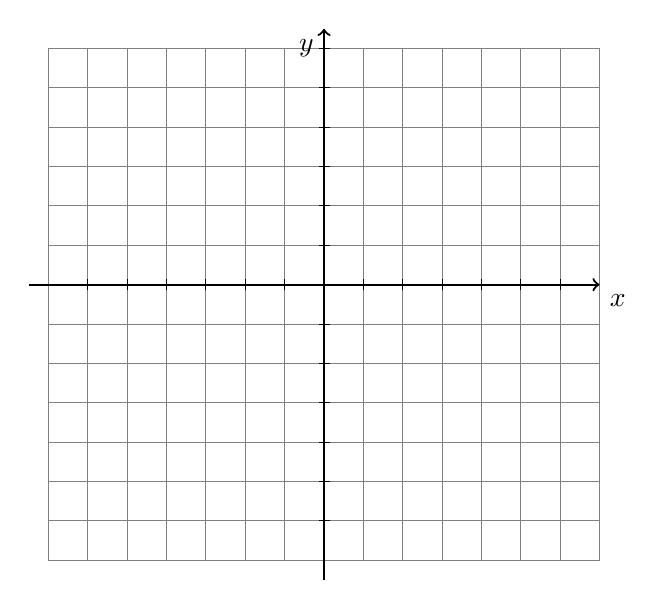
\begin{tikzpicture}[y=.5cm, x=0.5cm,font=\sffamily]
    %% ticks
    \draw[step = 1, gray] (-7,-7) grid (7,6);
    %% axis
    \draw[thick,->] (-7.5,0) -- coordinate (x axis mid) (7,0) node[anchor = north west] {$x$};
    \draw[thick,->] (0,-7.5) -- coordinate (y axis mid) (0,6.5) node[anchor = north east] {$y$};
    \foreach \y in {-6,-5,...,-1,1,2,...,6} {
      \draw (2pt, \y) -- (-2pt, \y);
    }
    \foreach \x in {-6,-5,...,-1,1,2,...,6} {
      \draw (\x,2pt) -- (\x,-2pt);
    }

\end{tikzpicture}



\item  Algebraically determine if $f(x)=-4x+1$ is one-to-one.

\vfill


\end{enumerate}



\vfill
\newpage

\item   Let $f(x)=5x+4$ and $\displaystyle g(x)=\frac{x-4}{5}$.\\
Use the theorem on inverse functions (function composition) to determine whether $f$ and $g$ are inverses.  Show every step.
\vfill


\item (1 point) Find the inverse function of $\displaystyle f(x)=\frac{8-x}{3}$.
\vfill




\end{enumerate}



